
\documentclass[12pt]{report}
\usepackage{graphicx,epstopdf}
\usepackage[absolute]{textpos}
\usepackage[english]{babel}
\usepackage[latin1]{inputenc}
\usepackage{amsmath,amsfonts}
\usepackage{natbib}
\usepackage{fancyhdr}
\usepackage{wrapfig}
\usepackage{float}
\usepackage[Conny]{fncychap}
\usepackage[usenames,dvipsnames]{color}
\usepackage{longtable}
\usepackage{multirow}
\usepackage{algorithmic}
\setcitestyle{numbers,open={[},close={]}}
\usepackage{epsfig}
\usepackage[official,right]{eurosym}
\usepackage{rotating}
\usepackage{hyperref}
\usepackage{rotating}
\hypersetup{pdfborder={0 0 0}}
\definecolor{light-gray}{gray}{0.95}
\usepackage[absolute]{textpos}
\usepackage[rounded]{syntax}
\usepackage{appendix}
\grammarparsep 1pt
\usepackage{xyling}
\usepackage{subfigure}
\usepackage{slashbox}
\usepackage{verbatim}
\usepackage{float}

\newfloat{Code}{H}{myc}
\allowdisplaybreaks

%EPS images snask

%\usepackage{epstopdf}
\newif\ifpdf
\ifx\pdfoutput\undefined
   \pdffalse
\else
   \pdfoutput=1
   \pdftrue
\fi
\ifpdf
   \usepackage{graphicx}
   \usepackage{epstopdf}
   \DeclareGraphicsRule{.eps}{pdf}{.pdf}{`epstopdf #1}
   \pdfcompresslevel=9
\else
   \usepackage{graphicx}
\fi
%eps image snask end
\epstopdfsetup{suffix=}

%semantic udtryk
\usepackage{turnstile}
%$\nststile{Bottom}{Top}$

%\usepackage[tt]{titlepic}


%LOL MARTIN!
%End lool martin

% C# lol?
\usepackage{listings}
% default words comes from lstlang1.sty
\lstset{language=Java,
  basicstyle=\ttfamily\footnotesize\bfseries,
  float,
  columns=flexible,
  morekeywords=[1]{TmdbAPI,TmdbMovie},
  %keywordstyle=[1]\sffamily,
  backgroundcolor=\color{light-gray},
  captionpos=b,
  frame=single,
  breaklines=true, 
  keywordstyle=\color{Blue},
  commentstyle=\color{Green},
  stringstyle=\color{Mahogany},
  showspaces=false,
  showstringspaces=false,
  numbers=left,                   % where to put the line-numbers
  numberstyle=\footnotesize,      % the size of the fonts that are used for the line-numbers
  stepnumber=1
  }
  \newenvironment{program}

%End c-sharp lol

\usepackage{url}

%% Define a new 'leo' style for the package that will use a smaller font.
\makeatletter
\def\url@leostyle{%
  \@ifundefined{selectfont}{\def\UrlFont{\sf}}{\def\UrlFont{\small\ttfamily}}}
\makeatother
%% Now actually use the newly defined style.
\urlstyle{leo}


\pagestyle{fancy}
\lhead{}

\newcommand{\code}[1]{\texttt{#1}}
\newcommand{\secref}{section \ref}
\newcommand{\appref}{appendix \ref}
\newcommand{\chapref}{chapter \ref}
\newcommand{\figref}{figure \ref}
\newcommand{\tabelref}{table \ref}
\newcommand{\listref}{listing \ref}
\renewcommand{\headrulewidth}{0.4pt}
\renewcommand{\footrulewidth}{0.4pt}

%Rasmus' kind of lol
\makeatletter
\newenvironment{Figure}{%
\par\addvspace{12pt plus2pt}%
\def\@captype{figure}%
}{%
\par\addvspace{12pt plus2pt}%
}%
\long\def\@makecaption#1#2{%
\vskip\abovecaptionskip
\sbox\@tempboxa{#1: #2}%
\ifdim \wd\@tempboxa >\hsize
#1: #2\par
\else
\global \@minipagefalse
\hb@xt@\hsize{\hfil\box\@tempboxa\hfil}%
\fi
\vskip\belowcaptionskip}
\makeatother
% Rasmus' kind of lol - stop

\setlength{\headheight}{15pt}

%titlepage image halløj
%\usepackage{eso-pic}
%\newcommand\BackgroundPic{
%\put(0,0){
%\parbox[b][\paperheight]{\paperwidth}{%
%\vfill
%\centering
%\includegraphics[width=\paperwidth,height=\paperheight,keepaspectratio]{Images/front-page.png}%
%\vfill
%}}}
%halløj end


%Jesper Stuff
\lstset{
	language=SQL,
  breaklines=true,                                     % line wrapping on
  frame=ltrb,
  framesep=5pt,
  basicstyle=\normalsize,
  keywordstyle=\ttfamily\color{OliveGreen},
  identifierstyle=\ttfamily\color{CadetBlue}\bfseries,
  commentstyle=\color{Brown},
  stringstyle=\ttfamily,
  showstringspaces=ture
}
\title{insert title here} %TODO
\author{os} %TODO

\begin{document}
\maketitle
\tableofcontents
	
	\chapter{Introduction}
\section{Motivation}
This is a student report written as part of a learning project.
We are required to comply with the study regulation, which states that the main focus of this semester is multi-project management and quality assurance in the form of requirements analysis, requirements management, and testing.\\
The goal is to create a comprehensive software system, across multiple project groups, in order to enhance our competences in analysis, design, implementation, and evaluation of software applications in regards to the system requirements. \cite{studyreg}

To create a comprehensive system that will be usable in real life scenarios, this project will build on top of a previous multi-group project and will also be built with the aim of having other students continue its development later.
Picking up and passing on application development within the system will make it possible to make them far more complex and by extend provide them with all of the necessary functions for them to be viable alternatives to tools that may exist already, as opposed to creating only ``single semester sized'' apps within the same system.\\
  
The multi-group project we are building on top of is aimed at creating a touch based tablet system to support children with autism and their guardians in every day scenarios.
In order to describe the context of this system we will in rest the introduction we will explore: 
\begin{description}
	\item[Target Group:] The group of people we hope to assist with our system.
	\item[Target Platform:] What platform will be the best for our system.
	\item[Development Method:] Which method that will serve us best in developing the system.
	\item[System Description:] The description of the areas we will be developing.
	\item[External Component Structure:]
\end{description}

\section{Target Group}
Our target group is both children and their guardians. These guardians have certain needs for special tools and gadgets that help to ease the communication between them and the children.

Five teachers and educators, who work with children, act as customers. They will provide requirements and information about the institutions' way of working to give us an insight into their daily struggles.

\subsection{Working with Children with ASD}
This section is based upon the statements of a woman with ASD \cite{autism.com}, explaining what it is like to live with ASD, and an interview with an educator at Birken, a special kindergarten for children (see \autoref{InterviewMette} for interview notes).

	People with ASD are often more visual in their way of thinking. Rather than visualizing thoughts in language and text, they do it in pictures or visual demonstrations. Pictures and symbols are therefore an essential part of the daily tools used by children and the people interacting with them. Also, children can have difficulties expressing themselves by writing or talking, and can often more easily use electronic devices to either type a sentence or show pictures, to communicate with people around them.
	Another characteristic of children is their perception of time. Some of them simply do not understand phrases like ``in a moment'' or ``soon'', they will need some kind of visual indicator that shows how long time they will have to wait.

Different communication tools for children with autism already exist, but many of them rely on a static database of pictures, and often these has to be printed on paper in order to use them as intended. Other tools, such as hourglasses of different sizes and colors, are also essential when working with children, and these tools are either brought around with the child, or a set is kept every place the child might go, e.g. being at an institution or at home.

There exists tools today which helps the guardians in their daily life, although -- as stated in Drazenko's quote -- none of them are cost-effective enough to be used throughout the institutions. From the quote, it is clear that there is a need for a more cost-effective solution.

\begin{quotation}
\textit{``The price of the existing solutions are not sufficiently low such that we can afford to buy and use them throughout the institution.''}\\ 
	\begin{flushright}
		- Drazenko Banjak, educator at Egebakken.
	\end{flushright}
\end{quotation}

\section{Target Platform}
In this learning project we have been imposed to develop applications for children with autism using the android platform[http://sict.moodle.aau.dk/file.php/628/SW6Android2012.pdf]. Android is an open-source platform and it is maintained by the \textit{Open Handset Alliance}(OHA) which is led by Google. Many companies are a part of the OHA, these companies contribute to the development with engineering resources. 

http://source.android.com/about/philosophy.html

\section{Development Method}

As a part of the study regulation we have been required to use the same development method in each individual group. Two methods have been considered, \textit{XP} (eXtreme Programming) \cite{XP}, and Scrum \cite{SCRUM}.

With the knowledge of both XP and Scrum, we decided in the multi project to use Scrum of Scrums, which is the use of Scrum nested in a larger Scrum project \cite{ScrumOfScrums}.

The reason for choosing Scrum of Scrums is that everyone, at all times, will be able to know what the vision of the project is, and how close every group is to achieving their individual goals of the vision.

Another element of the Scrum method is that a close contact with the customers is maintained. This helps keep the product backlog up to date and correctly prioritized. The customers are presented with the vision of the project, as well as showing the latest release when we have meetings with our customers.

We customized Scrum to fit our project. The changes are as follows:
\begin{itemize}
	\item The sprint length have been shortened to approximately 7 - 14 half days.
	\item Some degree of pair programming have been introduced.
	\item There is no project owner because this is a learning project.
	\item Everyone is attending the Scrum of Scrums meetings.
	\item The Scrum of Scrums meetings are only held once at sprint planning.
\end{itemize}

\section{Problem Definition}
In the multi project group, we have defined a preliminary problem statement, on which the individual project groups can expand.
The problem statement is worded as follows: 
\begin{quotation}
 ``How can we ease everyday life for children with autism and their guardians, through development on our target platform,
 while optimizing our development process by implementing a recognized project management method.''
\end{quotation}

This problem statement is necessarily vague to allow the individual groups some freedom in their projects, while we maintain the overall structure of the multi project, 
however there are limiting factors.
We are limited by resources and time available, as we are only working on this project for a single semester. However, all work done in this multi project
will be passed on to the next line of students, which means we can make a full system design and pass on anything we do not have the time or resources for.
This also requires that our work need to be of such quality that it is understandable by students of the same educational level as ourselves.
While not an actual limitation, we must adhere to the requirements of our customers, rather than working strictly with our own ideas as we may have been use to in previous projects.





  




		
\chapter{Development methods}
 %\section{Theory}
%	One of the goals of this semester is to show that we have knowledge in choosing and implementing different work methods and apply the method that we find most suited for our project. In order to do this one must first know the different methods before he/she will be able to choose the best suited. 

Different work methods can be put into two categories: Traditional and Agile.
The difference of traditional and agile methods are what they emphasizes the most.

Traditional methods puts big emphasize on analyzing the problem and create documentation of the analysis. The structure of a traditional method is therefore often split into phases, for instance the analysis phase or the implementation phase. Once a phase is done you move to the next phase. An example of this is the waterfall method. [put some example]

Agile methods on the other hand puts emphasis on analysis and documentation in a different way. Most agile methods utilizes an iteration driven work style. This means that you do all the phases over and over. This also means that you do not do the whole project at once. Instead you focus on getting a part of the system to work and then as more iterations are completed you add on to the system until the system is ready to be released. An example of this is the SCRUM method. [put some example]

Both approaches have strength and weaknesses. The traditional method features lots of documentation and analysis and so it is easier for others to understand if they are to develop further on the system. It also create a great overview of the whole system, and thus it is easier to estimate how long time it will take before the system is ready to ship. This makes traditional methods well suited for large projects. The agile method on the other hand implements the iteration driven approach. One of the great features of this approach is that you can correct errors and include things you might have forgotten relatively easy, because you just do it in the next iteration. 

One of the big drawbacks of the traditional method is that you cannot just go back a step, if you realize you have forgotten something or made an error. This is very costly because you have to do lots of steps over again. Another big issue with the traditional method is that the customers of the system might not always know what they want or need at the start of the development, but this is where you do all the analysis. The Agile method excels at this as you can present to your customers your current build and receive feedback that you might not have considered. 

The Work method that we find best suited for our project is an agile method. This is because in this semester we are working together with educators from institutions working with children with ASD. They will have requirements for our system so it is important that we are taking them into the project. It is also important that we choose a development method that have tools for managing bigger project groups as we are working as part of a bigger team to develop a system.

We have considered These following agile work methods:

\begin{itemize}
\item Scrum
\item Xp 
\end{itemize} 

In short Scrum is a method that emphasizes a self-directed and self-organizing team, each iteration is client driven meaning that the clients provides the requirements and features will be prioritized according to the clients needs.

XP emphasizes programming and testing. This means that there are very little documentation of the system other than the code. A simple design is preferred and the code is refactored with high frequency. This method requires high discipline since most planning is done orally.


    In our project it was required that all groups used the same development method to keep things simple. This means that the chosen development method may not be perfectly suited for every group, so while we have chosen the Scrum method we have also made some adjustments to fit it smoother for our group.

The key points of the adjustments are as follow

\begin{itemize}
\item The daily scrum meeting
\item The customer involvement
\item The sprint length
\item Incorporating key elements from Xp method
\end{itemize}

We, in our group, have not utilized the daily scrum meeting that is very typical and defining for the scrum method. The reason for this is that we are already sitting together in the same room. We also know each other well because we have worked together in earlier projects. If we felt like we needed to know anything about the other team members progress we could just ask. We simply did not feel the need to waste time every morning by stating the obvious. We see the daily scrum meeting as a tool for communication. We agree that communication is important to make a great product but we have used alternative ways to communicate.

Customer involvement have been a big focus in the multi project. However our group has been in a different situation than the others because our product has been the server which has little to no interest for the customers. Our biggest requirement providers has been the other groups. This has meant that we have not had a release after each sprint that was shown to the customer for feedback. This was only done once and only for the web interface. As mentioned in section [] a usability test was carried out to get a little more feedback from the customers. 

The sprint length has been modified because the ``number of days'' interval would be misleading because we have some days with lectures and others without. Instead we have define the term ``half days'' which covers either from 8.00 to 12.00 or from 12.00 to 16.00. This interval makes it possible to use days, with lectures covering up half the day, as working days. The sprint length has been dynamic and has been decided at each sprint start. A typical sprint length could be 14 half days which means the next 10 half days to occur. This could be a week without any lectures, or two weeks with lectures. 

There is a specific element associated with the Xp method that we felt the need to incorporate into Scrum, being the pair programming. We have incorporated this element because we find it well suited for programming while leaning. Because we had to learn a new programming language, Java servlet, that none of us had ealier experience in, pair programming helped us a lot in the beginning to quickly catch on.
  \section{Project Backlog}
    \label{sect:pback}
    \input{chapters/proBacklog.tex}

\chapter{Savannah} %TODO temp title
  \section{Requirements} %Martin
	\subsubsection{Initial Requirement gathering}
Requirement gathering was done in the multi project group in the very early stages of the project, but has also been updated as we have been progressing and showing our work to our customers.
In the initial stages we did semi-structured interviews of our customers, where the primary focus was understanding our target group and exploring any tools they currently have access to.
As mentioned the interviews were conducted in a semi-structured manner, we had a few questions%which..are missing?!?
but tried to let the interview run as an informal conversation where the customers could present their own ideas and visions of the project.

From these interviews we created an initial list of requirements for the multi project.
three interviews were done, with Mette and Christina from (ehhh) , Drazenko from (ehh), and Tove from Tale Instituttet(the speech center).
From the individual interviews we gathered a list of their individual ideas and visions and made a requirements list which groups later could refer back to.

\begin{itemize}
 \item Mette And Christina 
  \subitem Customizable software
  \subitem Ease of use, compared to current physical tools
  \subitem Emphasize visual stimuli
  \subitem Continuous stimuli 
 \item Drazenko
  \subitem Customizable software
  \subitem Visual abstract concept
  \subitem Emphasize visual stimuli
  \subitem Unambiguous
  \subitem Consistency/Structure
 \item Tove 
  \subitem Customizable software
  \subitem Engaging/Entertaining software
  \subitem Authentic/proper feedback or behavior
\end{itemize}

From the list of requirements of the individual customers, we identified the requirements which were common for all of them, and made a list of requirements which
should be common for all groups in the multi project.

\begin{itemize}
 \item Customizable software
  \subitem Some way to distinguish unique users on the same tablet is required, since people with autism have very different needs and have very different perceptions of the world.
  \subitem Customization should trump feature bloat.
 \item Emphasize visual stimuli
  \subitem Autistic people are visually over stimulated.
 \item Authentic/proper feedback or behavior.
\end{itemize}

These are all requirements set by our customers, however, since this system is dealing with potentially sensitive personal data, it is 
also a requirement that before it can be deployed in a real world situation, that all transmissions are done via a secure connection. %incomplete 
  \section{Database}
  	%databaseintro.tex
To facilitate profile management, a database has been designed and implemented. This section describes the process of the database creation.
    \subsection{Design}
    	%datadasedesign.tex
The database is designed in MySQL 5.1.61, and resembles the local database created by Oasis -- the only difference is, that the Savannah database has two extra attributes in the \code{AuthUsers} table: \code{username} and \code{password}. The reason for this is that while all GIRAF apps running on the Android platform uses QR-codes for user authentication, this is not a feasible solution for the web interface, as it can not be assumed that every user has a webcam conneceted to the computer.

\subsubsection{Requirements}
The requirements for the database has been provided by the other project groups, and are as follows:

\begin{itemize} % TODO ohnoes..punktummer
	\item All users must be able to login with a QR-code
	\item Each department must also be able to login
	\item All users must be linked to at least one department
	\item All guardians must be able to be linked to at least one child.
	\item All parents must be able to be linked to at least one child.
	\item All users must be able to have to their selected apps
	\item All users must be able to access their own pictures, and all public pictures
	\item All departments must be able to access all public pictures
	\item All pictures needs to be able to be linked to tags
	\item Pictures must be able to be linked with audio and vice versa
	\item A department must be able to have a subdepartment\footnote{Example: Birken has two departments, at two different addresses, both these subdepartments needs to be linked with Birken as a superdepartment}
\end{itemize}

\subsubsection*{Diagram} %TODO fix overskrift
A diagram has been made to get a overview of the different tables and their relations. This diagram is designed in DIA\cite{Dia}, and can be seen in \autoref{fig:DiaDesign}.

\begin{figure}[htbp]
	\centering
		\includegraphics[width=1.00\textwidth]{images/DiaDesign.png}
	\caption{Dia diagram of the database}
	\label{fig:DiaDesign}
\end{figure}

Although the diagram in \autoref{fig:DiaDesign} does not meet the conventions of database diagrams, it does provide a good view of the different tables, and the relations: Foreign keys points to where the value is fetched from.

\subsubsection{Normal Form}
To prevent modification anomalies in the database, it can be normalized. This becomes important when a table is dealing with functional dependencies. The solution is to remove the dependicies from the table to another, e.g. split a table into two new tables. An example of this is shown in \autoref{tab:nonNormalizedExample} and \autoref{tab:NormalizedDatabaseExample}.

\begin{table}[htbp]
	\centering
		\begin{tabular}{|c|c|c|}
		\hline
		 \multicolumn{3}{|c|}{SALES}\\
		\multicolumn{1}{|c}{Customer\_ID} & \multicolumn{1}{c}{Product} & \multicolumn{1}{c|}{Price} \\
		\hline
		1001 & Laundry detergent & 12 \\ \hline
		1007 & Toothpaste & 3 \\ \hline
		1010 & Chlorine bleach & 4 \\ \hline
		1024 & Toothpaste & 3\\	\hline
		\end{tabular}
	\caption{Non-normalized database\cite[p. 114]{sqlForDummies}}
	\label{tab:nonNormalizedExample}
\end{table}

The problem in \autoref{tab:nonNormalizedExample} is that if customer 1001 is removed from the table, not only is his product removed, but the fact that Laundry detergent costs 12\$ is also lost. A way to prevent this, is to split the table into two tables, as seen in \autoref{tab:NormalizedDatabaseExample}

\begin{table}[htbp]
	\centering
		\begin{tabular}{c c}
			\begin{tabular}{|c|c|}
				\hline
		 		\multicolumn{2}{|c|}{CUST\_PURCH} \\
		 		\multicolumn{1}{|c}{Customer\_ID} & \multicolumn{1}{c|}{Product} \\
		 		\hline
		 		1001 & Laundry detergent \\ \hline
		 		1007 & Toothpaste \\ \hline
		 		1010 & Chlorine bleach \\ \hline
		 		1024 & Toothpaste \\ \hline
			\end{tabular}
		&
			\begin{tabular}{|c|c|}
				\hline
				\multicolumn{2}{|c|}{PROD\_PRICE} \\
				\multicolumn{1}{|c}{Product} & \multicolumn{1}{c|}{Price} \\
				\hline
				Laundry detergent & 12 \\ \hline
				Toothpaste & 3 \\ \hline
				Chlorine bleach & 4 \\ \hline
			\end{tabular}
		\end{tabular}
	\caption{Normalized database example\cite[p 115]{sqlForDummies}}
	\label{tab:NormalizedDatabaseExample}
	\end{table}

As seen in \autoref{tab:NormalizedDatabaseExample} the table \code{CUST\_PURCH} now only deals with the customer, and thus it is now possible to remove a customer from the system, without loosing the product's price.

There are several degrees of normal form for a database, here the focus is on the first three: first, second, and third normal form.

\subsubsection{First Normal Form (1NF)}
The example in \autoref{tab:NormalizedDatabaseExample}, is an example of 1NF. To achieve this the following qualities must apply\cite[p. 116]{sqlForDummies}:
\begin{itemize}
	\item Each cell (intersection of a row and a column) of the table must have only a single value.
	\item Each column must have a unique name.
	\item No two rows may be identical (that is, each row must be unique).
	\item Each column contains data for a single attribute of the thing it's describing.
\end{itemize}

As seen in \autoref{fig:DiaDesign} the Savannah database fullfills the qualities of 1NF, and thus is 1NF.

\subsubsection{Second Normal Form (2NF)}
For a database to be in 2NF it is required that if a table contains a composite key, all other attributes in the table must be depended on the entire key.
Furthermore \cite[p. 117]{sqlForDummies} states:
\begin{quotation}
...every
relation that is in 1NF with a single attribute key is automatically in second
normal form.
\end{quotation}
As this is the case in the Savannah database, it is in 2NF.

\subsubsection{Third Normal Form (3NF)}
For a database to be in 3NF, it is required that there are no transitive dependency\footnote{A transitive dependency occurs when one attribute depends on a second
attribute, which depends on a third attribute. Deletions in a table with such a
dependency can cause unwanted information loss. \cite[p. 118]{sqlForDummies}}.
As seen in \autoref{fig:DiaDesign} Savannah's database lives up to this quality, as there are no transitive dependencies within any of the tables. A good example of this is the handling of a profile's access to apps: When the app is removed from the profile it is done in the \code{ListOfApps} table, and thus only the relation is removed, and the specific app is still available in the system. This means the Savannah database is in 3NF.



\subsubsection*{Constraints}
\label{databaseRules}
To provide the security needed in the system, several constraints need to apply for the database:
\begin{itemize}
	\item The \code{Profile}$\rightarrow$\code{AuthUsers} relation must be one-to-one, as one user from the \code{AuthUsers} can only have one profile in the system
	\item The \code{Department}$\rightarrow$\code{AuthUsers} relation must be one-to-one, as one department from the \code{AuthUsers} can only be one department in the system
	\item The \code{idUser} attribute in \code{AuthUsers} must be unique.
	\item The \code{username} attribute in \code{AuthUsers} must be unique
	\item It must be possible to distinguish between users and departments in the \code{AuthUsers} table
	\item It must be possible to distinguish between children, parents and guardians in the \code{Profile} table
\end{itemize}

These constraints will be implemented through the use of SQL scripts and Java code in \textbf{REF TIL SECTION} %TODO
    \subsection{Implementation}
    	%databaseimpl.tex
The implementation of the MySQL database is done in MySQL Workbench 5.2.40 which is a GUI tool that provides a large set of features for various purposes.

Due to the dependencies of the various tables, the order of how the need to be created is quite strict. 
The code to create the tables is found in the appendix \autoref{MySQLcode}. 
To make sure the ``username'' and ``userID'' follows the previously stated rules, both fields has been made \verb+UNIQUE NOT NULL+ and the ``userID'' furthermore has \verb+AUTO_INCREMENT+ as seen in \autoref{createAuthUsers}. 
This makes sure there can be no one with the same ``username'' or ``userID'' and the ``userID'' will automatic increase when new data is inserted. 
This also guarantees a one-to-one relation between both ``Profile'' and ``AuthUsers'' and ``Departments'' and ``AuthUsers''. 
To be able to distinguish between ``Department'' and ``Profiles'' a filed called \verb+aRole+ is used. 
This is a int and will hold a number, which will be used at software level to do the distinguishing. The same applies for the distinguishing in ``Profile'' (code shown in \autoref{createProfile}), here a field called \verb+pRole+ holds an int, which again will be used at software level.

The MySQL Workbench provides the functionality to create a ERR diagram form an existing database, this diagram is shown in \autoref{fig:workbenchRight}. The diagram is con completely as MySQL workbench creates it, the real is shown in the appendix \autoref{errDiagram}. But this is a error in the software; as seen in the diagram, the tool generates the ``Profiles''$\rightarrow$''AuthUsers'' as a one-to-many relation. This however, is not possible since the ``idUser'' field in ``AuthUsers'' is unique (as seen in \autoref{createAuthUsers}), the same goes for both ``Departments'' and ``Medias''.

\begin{figure}
	\centering
		\includegraphics[width=1.00\textwidth]{images/workbenchRight.png}
	\caption{The ERR diagram}
	\label{fig:workbenchRight}
\end{figure}


To make the deletion of data easy, many of the filed in the tables has the constraint \verb+ON DELETE CASCADE+. This can be ``dangerous'', as side-effects can result in unintended data will be deleted. To makes sure no unintended data will be deleted, the software level implementation needs to warn the user when deleting data. Furthermore an analysis has been made to argue for which fileds can have this constraint. The following tables and fields has the cascade constraint: 
\begin{verbatim}
``Profiles''.''idProfile'', 
``ListOfApps''.''idProfile'', 
``HasDepartment''.''idProfile'', 
``HasGuardian''.''idGuardian'', 
``HasGuardian''.''idChild'', 
``Media''.''OwnerID'', 
``HasTag''.''idMedia'', 
``HasLink''.''idMedia'', 
``HasLink''.''idSubMedia'',
''MediaProfileAccess''.''idProfile''.
\end{verbatim}

\subsubsection*{Use case}
 An use case of the constraint is:
\begin{quotation}
``A user ``Jesper'' wishes to delete his entire profile''
\end{quotation}
What will happen is:
\begin{enumerate}
	\item A deletion of the ``userID'' in ``AuthUsers'' is executed
	\item The relation between ``AuthUsers'' and ``Profiles'' will delete the profile
	\item The relation between ``Profiles'' and ``HasGuardian'' will delete all fields where the ``userID'' is either ``idGuardian'' or ``idChild''
	\item The relation between ``AuthUsers'' and ``Media'' will delete all fields where ``idUser'' is the owner
	\item The relation between ``Media'' and ``HasTag'' will delete all fields where ``HasTags''.``idMedia'' equals ``idMedia''
	\item The relation between ``Media'' and ``HasLink'' will delete all fields where ``HasLink''.''idMedia'' or ``HasLink''.''idSubMedia'' equals ``idMedia''
\end{enumerate}


    \subsection{Test}

  \section{Web Interface}
   \label{sect:webInterface}
     \subsection{Programming language}
      %programminglanguage.tex
To be able to provide the desired functionality form the web interface, a dynamic web page needs to be created. There are several different programming languages to choose from. Some of the most common are ASP.net, PHP and Java servlets. Due to the fact that ASP.net is not open source (REF til asp.net/terms-of-use), and the project is, this is not a feasible choice. This section will do a deeper analysis of PHP and Java servlets, to argue for the best choice of programming language.

\subsubsection{PHP}

\subsubsection{Java Servlets}
     \subsection{Implementation}
     \subsection{Test}
		In this section we have described the tests we have made for our web interface. First we present our results from the usability test and then we present the test cases and their results.

\subsubsection{Usability Test}

Our usability test was carried out using the IDA. The results are as shown in \autoref{tab:results}

\begin{table}[H]
	\scriptsize
	\centering
	\begin{tabular}{|p{7cm}|r|r|}
		\hline
		Error & Frequency & Category \\
		\hline
		\hline
		Create a profile was difficult and counter intuitive & 3 & Serious \\ \hline
		The home button was only on some sites and confuses the user & 5 & Serious \\ \hline
		/imagenull would appear for no reason when a user was created & 3 & Cosmetic \\ \hline
		HTTP errors during the test & 5 & Critical \\ \hline
		Access to apps caused confusion, the user could not figure out what it was used for & 5 & Cosmetic \\ \hline
		Choose file was not further specified and caused confusion & 3 & Cosmetic \\ \hline
		GUI size was not filling up the whole screen which some of the test subjects found inconvenient & 2 & Cosmetic \\ \hline
		QR-code page misunderstanding home link & 3 & Cosmetic \\ \hline
		Add guardian to child was counter intuitive & 3 & Critical \\ \hline
		Edit profile made the users believe that they had to change password every time & 2 & Serious \\ \hline
		When logging in on child's profile as guardian the dropdown menu was confusing & 4 & Serious \\ \hline
		The user was confused of what to do after login & 1 & Cosmetic \\ \hline
		Edit/add picture was confusing & 3 & Serious \\ \hline
		The phone number was required but this is not the situation in reality & 5 & Critical \\ \hline
		Missing caption for choosing role causes confusion & 1 & Cosmetic \\ \hline
		The test subject was unsure which tags corresponded to which check-box & 2 & Critical \\ \hline
		Confusing, too many options & 1 & Serious \\ \hline
		The test subject tried to login as one of the predefined users because they thought it was their profile & 2 & Cosmetic \\ \hline
		The user lost the overview & 5 & Serious \\ \hline
		The user was not sure which pictures were public when asked to delete a public picture & 1 & Cosmetic \\ \hline
		When deleting pictures, the tags in brackets caused confusion and the text fields implied that you could write in them which is not the case & 1 & Cosmetic \\ \hline
		The test subject was unsure how to get back from the audio page & 1 & Cosmetic \\
		\hline
	\end{tabular}
	\caption{Results of the usability test}
	\label{tab:results}
\end{table}

In summation: 11 errors were defined as cosmetic, 7 as serious, and 4 as critical. \\

The critical errors were that the page broke down with an error. another critical error was that a phone number was required for a child, while it should be optional.
This is a requirement that has not been implemented, because we have not gotten the request before the test.
When prompted to add a guardian to a child there was great confusion of how to do that.
The reason is mainly because it is not placed in an intuitive place, and the test subjects had to get help from the test monitor.
The last critical error was the tags selection. The problem was that the user did not know, if a checkbox was assigned to the caption above or below. While this seems as a cosmetic or serious problem, at worst the system crashed. We have not been able to recreate this crash so we have rated the problem as critical although the system might not crash.

The rest of the problems found in the test was primarily things missing, bad layout, or misplaced functionality.
Missing things include ``back'' or ``home'' options from certain pages or captions that tells the user what certain fields do when filling out formulas. Bad layout is the main reason for confusion when using the system, this could be too much information presented to the user at once.
Misplaced functionality includes the placement of the profile list on the main page which a lot of users thought had to do with editing and adding profiles leading to big confusion. 

  \section{serverside} %TODO temp title
    The following chapter concerns the design and implementation of the server side software for savannah and the sw6ml language.
    \subsection{Architechture and Design}
      \label{sect:ssArchAndDesign}
      \subsubsection*{Architecture}
An overall design and architecture was created in the early sprints of the project.
 The server side software is different from the rest of the software made in the multi project group, as the customers will never actually see it in action. It works as intended if they never notice it is there.
Almost all requirements from our customers concern the user interface and general feel of the GIRAF apps. In regards to the server software, it is the requirements of the multi project that are of interest,
in particular Oasis, as their responsibility is to link the GIRAF apps to Savannah.

The GIRAF system is designed in such a way that it deploys with two databases: Savannah - our project, a global database for a full deployment unit, and Oasis - or localDB, a local database which exists only
on the mobile devices, which has an almost identical schema to Savannah's database.
Rather than having Oasis query the global database directly, it was decided to implement access to both the databases through a software layer, as shown in \autoref{fig:softwareLayers}.
The pros and cons of this seemingly redundant software layer was considered, see \autoref{table:proconSoftwareLayers}

\begin{figure}[H]
	\centering
		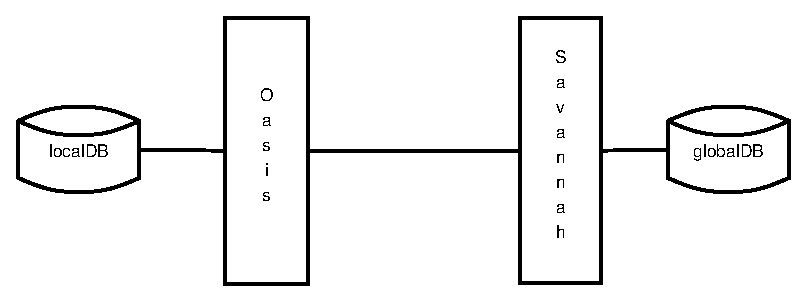
\includegraphics[scale=1]{images/softwareLayers}
	\caption{Software layers}
	\label{fig:softwareLayers}
\end{figure}

\begin{table}[H]
  \begin{center}
    \begin{tabular}{c|c}
    Pros                   &             Cons \\
    \hline
    More flexibilty        & Higher complexity\\
    Independent DB updates & Lower performance\\
    \end{tabular}
    \caption{Pros and cons of an extra software layer between the databases}
    \label{table:proconSoftwareLayers}
  \end{center}
\end{table}

Having an extra software layer between the databases means we can alter the global and local databases independently of each other. By providing software with methods for extracting specific
details from Savannah, like full profiles, Oasis does not have worry about Savannah's internal database schema. The downside of this is that the complexity inevitably will be higher, and performance
will be lower. The performance issue is not critical though, since the perceived performance of the system will be dominated by the bandwidth of the mobile devices. 
The communication between the software layers will be facilitated by the sw6ml XML language, presented in \autoref{sw6ml}

Savannah has a three layered internal architecture, show in \autoref{figure:savaArch}.

\begin{figure}[H]
  \centering
    \includegraphics{images/savaArch}
  \caption{Savannah's architecture}
  \label{figure:savaArch}
\end{figure}

A short description of each layer's responsibilities follows:

\begin{description}
 \item[Services] The services layers consists of the services that we provide to external users. We have considered two services to include, which are an API for creating transmissions packages	 		that Savannah understands, and the web interface discussed in \autoref{sect:webInterface}.
 \item[Communication] The communication layer consists of the IO package of the server side software, which handles retrieval and responding.
 \item[Service] The service layer consists of event handling, query handling and the building of sw6ml documents.
\end{description}


\subsubsection*{Design}
The overall server software is designed around a producer-consumer pattern, where Oasis acts as the producer through Savannah's IO layer.
Request or commit packages sent to Savannah will be processed by the \code{IOHandler}, which will add an event to the \code{EventQueue}. The consumer is the server itself, which will remove events from the queue and process its content, being it a request or a commit. Using a queue based design was chosen for the sake of simplicity. The project is a part of learning process, and building a server with concurrent event handling was down prioritized versus a simpler server, which would allow us to gain experience and still meet the requirements of the study regulations.
 A draft of the design for the server can be seen in \autoref{figure:serverMockup}. This diagram represents the general idea and flow of the server, and should not be understood as formal technical specification.
\begin{figure}[H]
 \centering
  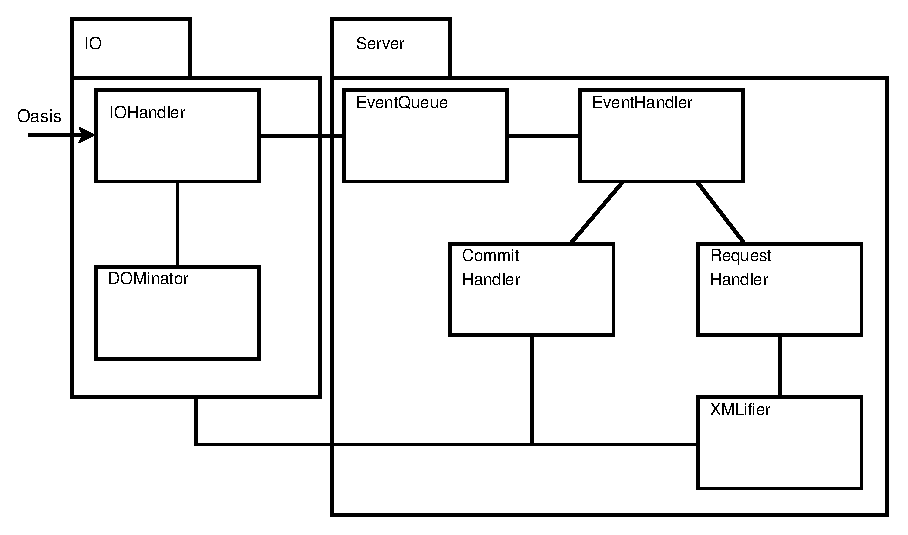
\includegraphics[scale=1]{images/savaIniDesign}
 \caption{Savannah server draft}
 \label{figure:serverMockup}
\end{figure}

      \subsubsection{sw6ml} %Martin
         \label{sw6ml}
	  %Introduction
In order to facilitate consistent data transfer between the global database and localDB, we have designed an XML language which mimics
the schema of the database. We have chosen to use XML as it is a recognized standard, with a wide array of tools available, in particular JDOM\cite{www.jdom.org}.
JDOM is a light weight implementation of SAX and the Data Object Model(DOM) for java, which allows seamless integration of XML, with support for XPath and XSLT.
In \autoref{sw6mlusage} a short usage documentation for sw6ml is provided. sw6ml is defined with XML schema.

\subsubsection{Language Design}

The sw6ml language consists of a number of primary elements which reflect the tables in the database, each of these elements accepts any number of ENTRY elements that tell
the server what action is should do with the incomming data.
in \autoref{code:sw6mlExample01} a short example of legit sw6ml syntax for adding a row to the AuthUsers table and deleting a row with the idUser table attribute equal to 2 is shown.
The \code{<AuthUsers>..content..</AuthUsers>} element identify the table on which we want to make changes, the following \code{<Entry>..content..</Entry>} elements
define what row and what kind of action, through the \code{action="foo"} xml attribute, should be done on the row. 

\begin{figure}[H]
\begin{lstlisting}[label=code:sw6mlExample01,caption=Example of sw6ml syntax]
 <AuthUsers>
    <Entry action="create">
      <certificate type="string">This is a certificate</certificate>
      <idUser type="int">1</idUser>
      <arole type="int">1</arole>
      <username type="string">mette</username>
      <password type="string">obfuscated</password>
    </Entry>
    <Entry action="delete">
      <idUser type="int">2</idUser>
    </Entry>
  </AuthUsers>
\end{lstlisting}
\end{figure}
The \code{action="foo"} xml attribute has four legal types corresponding to the CRUD profile actions, create, read, update, and delete, shown in \autoref{code:sw6mlCrud}.
Contained in the  \code{<Entry action="crud_type`">..content..</Entry>} element is a series of 0 or more elements corresponding to the table schema of, in this case, the AuthUsers table.
It takes zero or more of the table attributes in a row, since not all table attributes are needed for all actions, as an example delete only requires the unique identifier of the table and
updates will only need the unique identifier and the table attribute being updated.
\begin{figure}[H]
\begin{lstlisting}[label=code:sw6mlCrud,caption=sw6ml crud simple type]
 <xs:simpleType name="crud">
  <xs:restriction base="xs:string">
    <xs:enumeration value="create"/>
    <xs:enumeration value="read"/>
    <xs:enumeration value="update"/>
    <xs:enumeration value="delete"/>
  </xs:restriction>
</xs:simpleType>
\end{lstlisting}
\end{figure}

\subsubsection{Documentation}
\label{sw6mlusage}
To use the current version of sw6ml and savannah together it is essential to know the elements required from the different crud types.
while XML schema provides advanced features for dynamic languages, sw6ml int its current version, is a primitive language consisting of simple types and sequences.
this is however all that is needed, with a few assertions on the format server side.

\autoref{code:sw6mlformal} show the formal structure of a sw6ml document.
\begin{figure}[H]
\begin{lstlisting}[label=code:sw6mlformal,caption=root and table elements]
<sw6ml> 
  <table_element_1>
    <Entry action="crud_type">
      <table_element_1_attribute_1/>
	...
      <table_element_1_attribute_n/>
    </Entry>
  </table_element_n>
  ...
  <table_element_n>
    <Entry action="crud_type">
      <table_element_n_attribute_1/>
	...
      <table_element_n_attribute_n/>
    </Entry>
  </table_element>
</sw6ml>
\end{lstlisting}
\end{figure}

following is a short description of the setup of the \code{<Entry>} element for each crud type.

\begin{description}
 \item[create] creates a new row in the database: All attributes from the database schema is required, if no value exists, use null. See \autoref{code:sw6mlExample01} for an example.
 \item[update] Updates a field in a row, Required in this order: Unique identifier of the row, Attribute to be updated. See \autoref{code:sw6mlExample02} for an example.
 \item[delete] Deletes a row in the able: Only the unique identier is required. See \autoref{code:sw6mlExample01} for an example.
 \item[read]   Read is only used in xml which is send back on a request to the server, and thus require no special formatting.
\end{description}

Notice the \code{<row_attribute type="bar">..</..>} xml attribute, legal types are \code{string} or \code{int}, if the data type of the row attribute is a string or any other type requiring apostrophes
in a sql query, use \code{string}, for anything else use \code{int}.

\begin{lstlisting}[label=code:sw6mlExample02,caption="sw6ml Update syntax example]
 <Entry action="update">
   <unique_identifier type="bar">foo</unique_identifier>
   <attribute_to_be_updated type="bar">newValue</attribute_to_be_updated>
 </Entry>
\end{lstlisting}

The sw6ml schema can be found on the project repository together with an valid sw6ml document
Full path: \url{http://code.google.com/p/sw6-2012/source/browse/random_group_stuff/Group_server/xml/sw6_schema.xsd}
and \url{http://code.google.com/p/sw6-2012/source/browse/random_group_stuff/Group_server/xml/sw6_example.xml} %TODO fix this document before handin;-)






	  
    \subsection{Implementation}
      \subsubsection{Input handling} %Thorbjørn
		When the server starts it will execute a method called \code{listen()} that listens for any connections, see \autoref{code:listen}.
Whenever any \code{java.net.Socket} connects to the server, the \code{listen()} method will create a new \code{CommunicationThread}.
This thread will then read the information in the \code{Socket}'s \code{java.io.InputStream} and depending on the connection type (commit event, request event or ping) it will deal with it appropriately.

\lstinputlisting[language=Java,label=code:listen,caption=Method: \code{listen()}]{code/IOHandler-listen.txt}

In the following we will explain how the different types of connections are processed by the system.


\subsubsection*{Ping}
Diagram ledger: (see \autoref{fig:IOLedger})\newline
The uppermost port is used to indicate input and the lowermost port is used to indicate output. The arrows indicate which way the information is forwarded in the system. Any arrows leading to and fro a component, and not from an input or output port, are to be executed first.	\newline
\begin{figure}[H]
	\centering
		\includegraphics[scale=0.40]{images/ledger} %FIXME epstopdf package fucker, har ændret noget her
	\caption{Ledger for diagrams}
	\label{fig:IOLedger}
\end{figure}

%	The \newlines are to prevent the words from "running" out of the page - don't know why this happens :(
% This has been tested with   \texttt{arg} and \code{arg}
Figure~\ref{fig:IOPing} is a model of how a ping is process by the server. The \code{Connection} component sends output, in this case a ping event, to the server. In the server this is received by the \code{IOHandler}, which creates a new \newline \code{CommunicationThread}.
The \code{CommunicationThread} will then use the \newline \code{TransmissionHandler} to determine if the input is of the type commit, request or ping.
In this case the input is of the type ping, and it will just directly respond to the caller (connection). 
More information on these classes can be found in \autoref{fig:app:IOHandler}, \autoref{fig:app:Connection}, and \autoref{fig:app:TransmissionHandler}.
\begin{figure}[htbp]
	\centering
          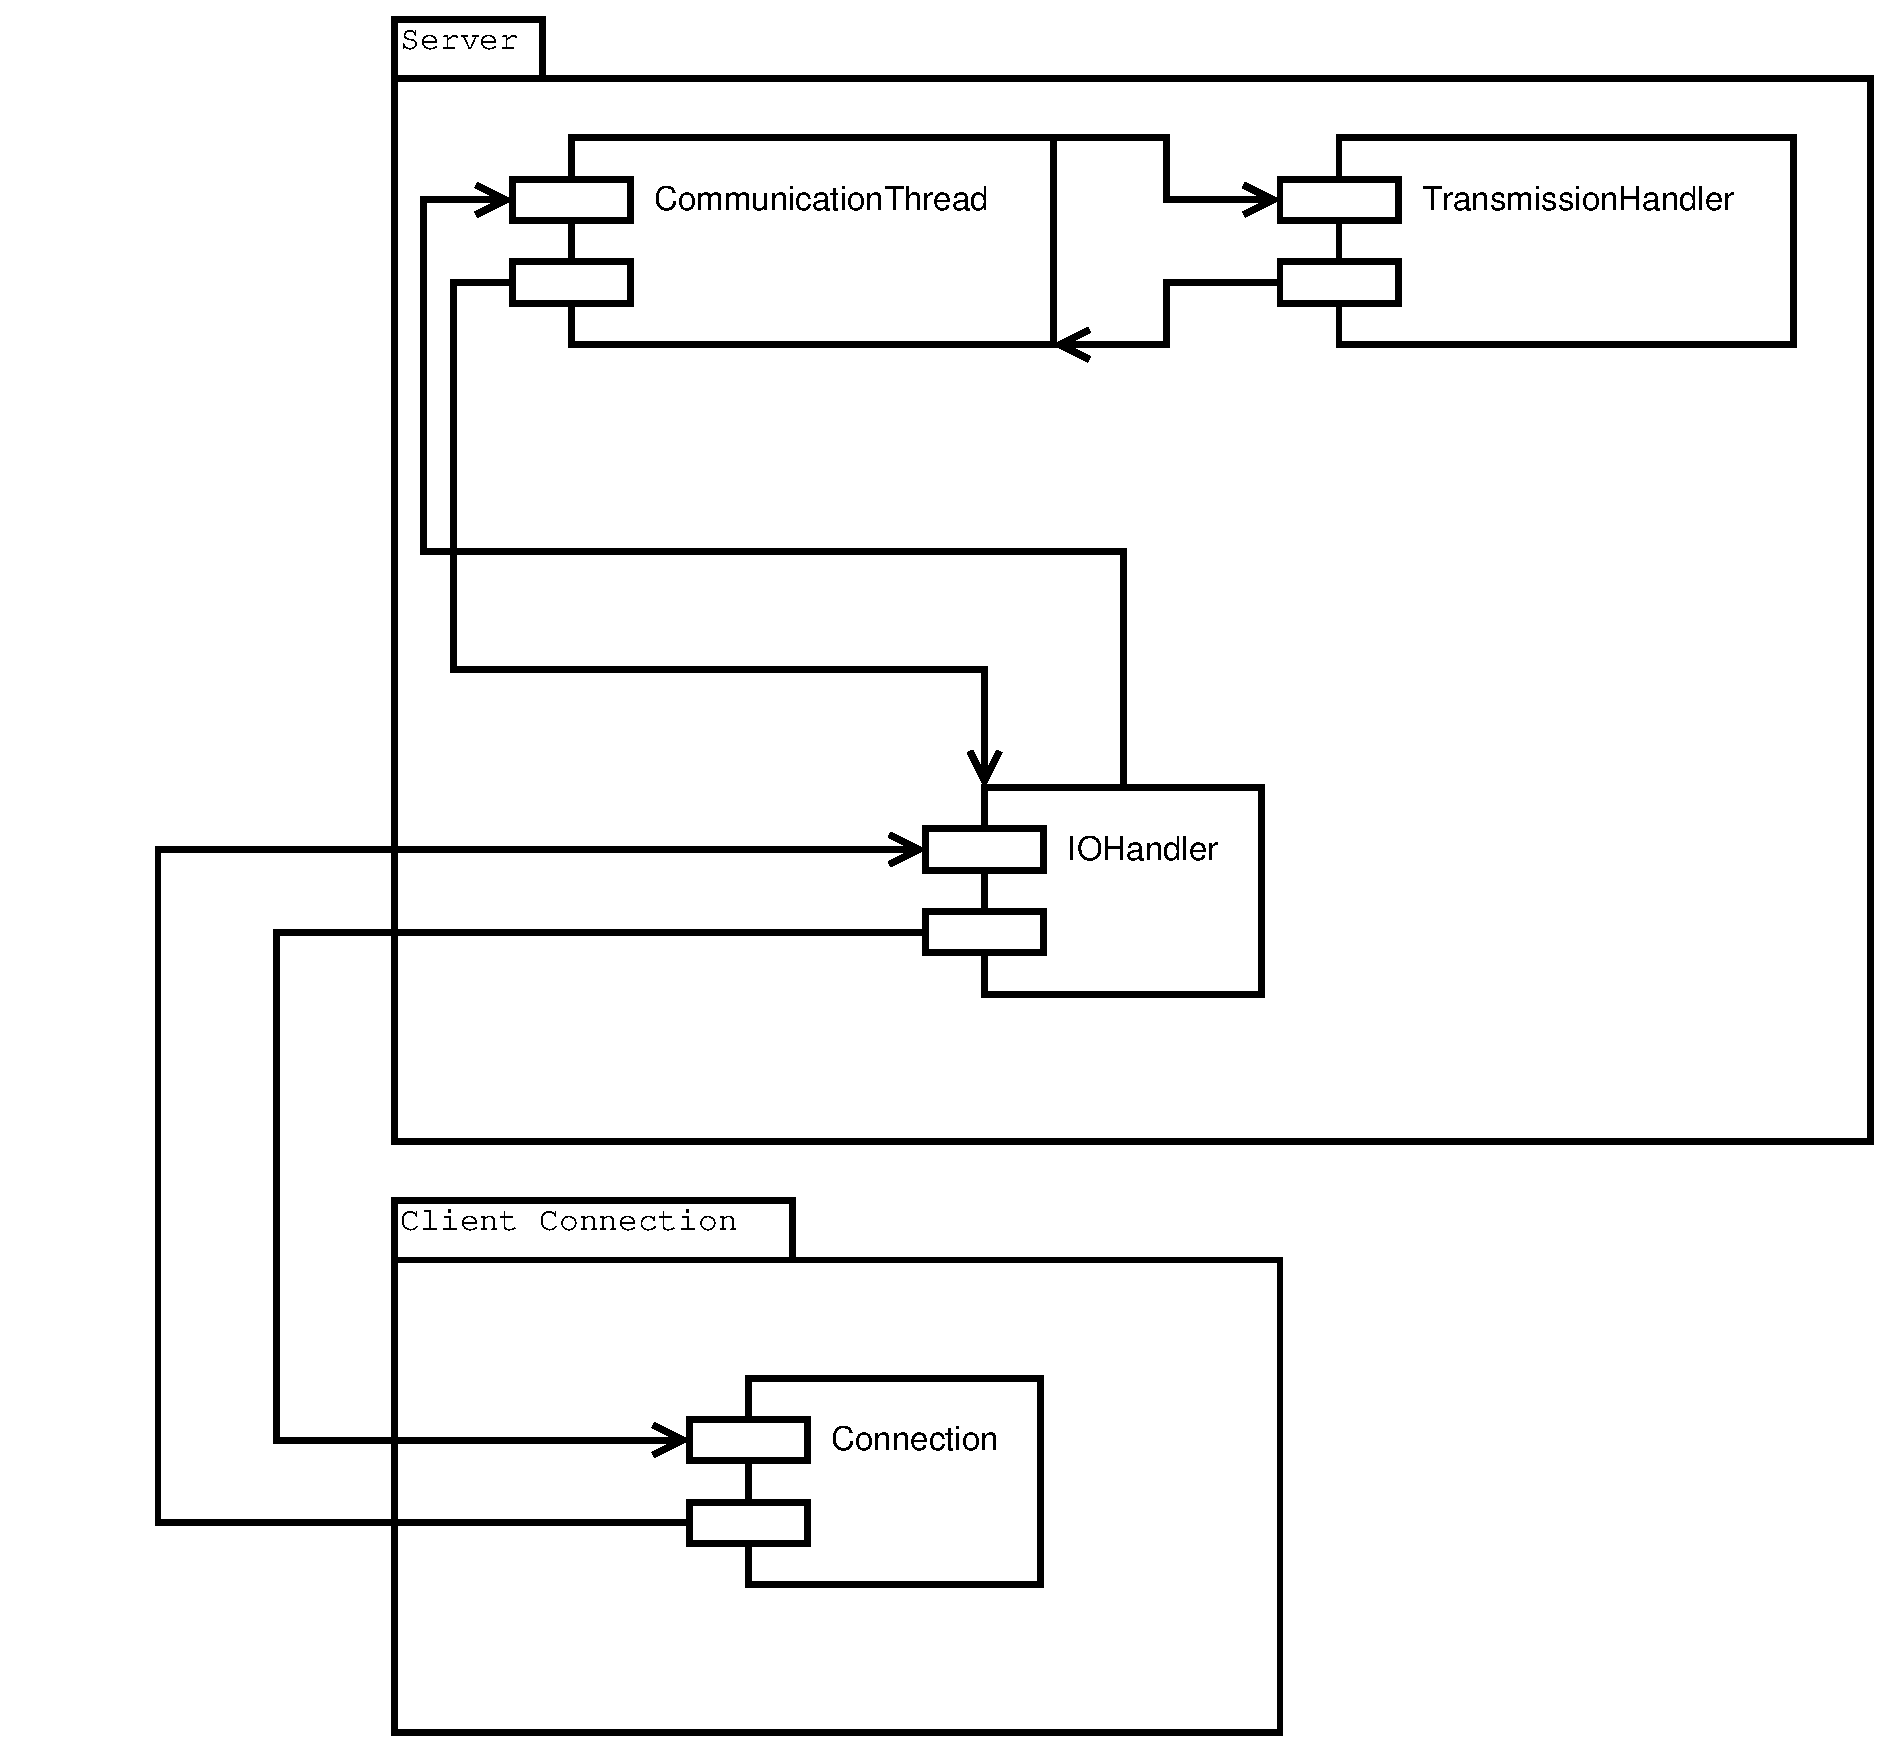
\includegraphics[scale=0.30]{images/ping}%FIXME epstopdf packager fucker, har ændret til at bruge de generede pdf filer direkte
	\caption{A diagram illustrating how a ping is processed.} 
	\label{fig:IOPing}
\end{figure}

%	The \newlines are to prevent the words from "running" out of the page - don't know why this happens :(
% This has been tested with   \texttt{arg} and \code{arg}
The reason for this implementation is that Java only supports two types of sockets: stream based (TCP -- \code{java.net.Socket} and \code{java.net.ServerSocket}) and datagram based ones (UDP -- \code{java.net.DatagramSocket} \newline and \code{java.net.MulticastSocket})\cite{ICMP}\cite{javaNET}.
However an implementation of ping would require the use of ICMP(Internet Control Message Protocol) ping, and since this is not possible we have implemted our own ping-like function.
%chose to implement a ping at a software level, rather than as a protocol.


\subsubsection*{Commit and Request}
For a connection of type commit or request, the procedure is almost the same. However, when the \code{CommunicationThread} has been created and its \code{TransmissionHandler} has determine the type of the connection, it will opposite for the ping, create a new event corresponding to the type and send it to the \code{EventHandler}, see \autoref{fig:IOCR}.
First when the \code{EventHandler} is done processing the event, will the server respond to the connector.
To see how the \code{EventHandler} processes the given queries see \autoref{QQHandling}.

\begin{figure}[htbp]
	\centering
		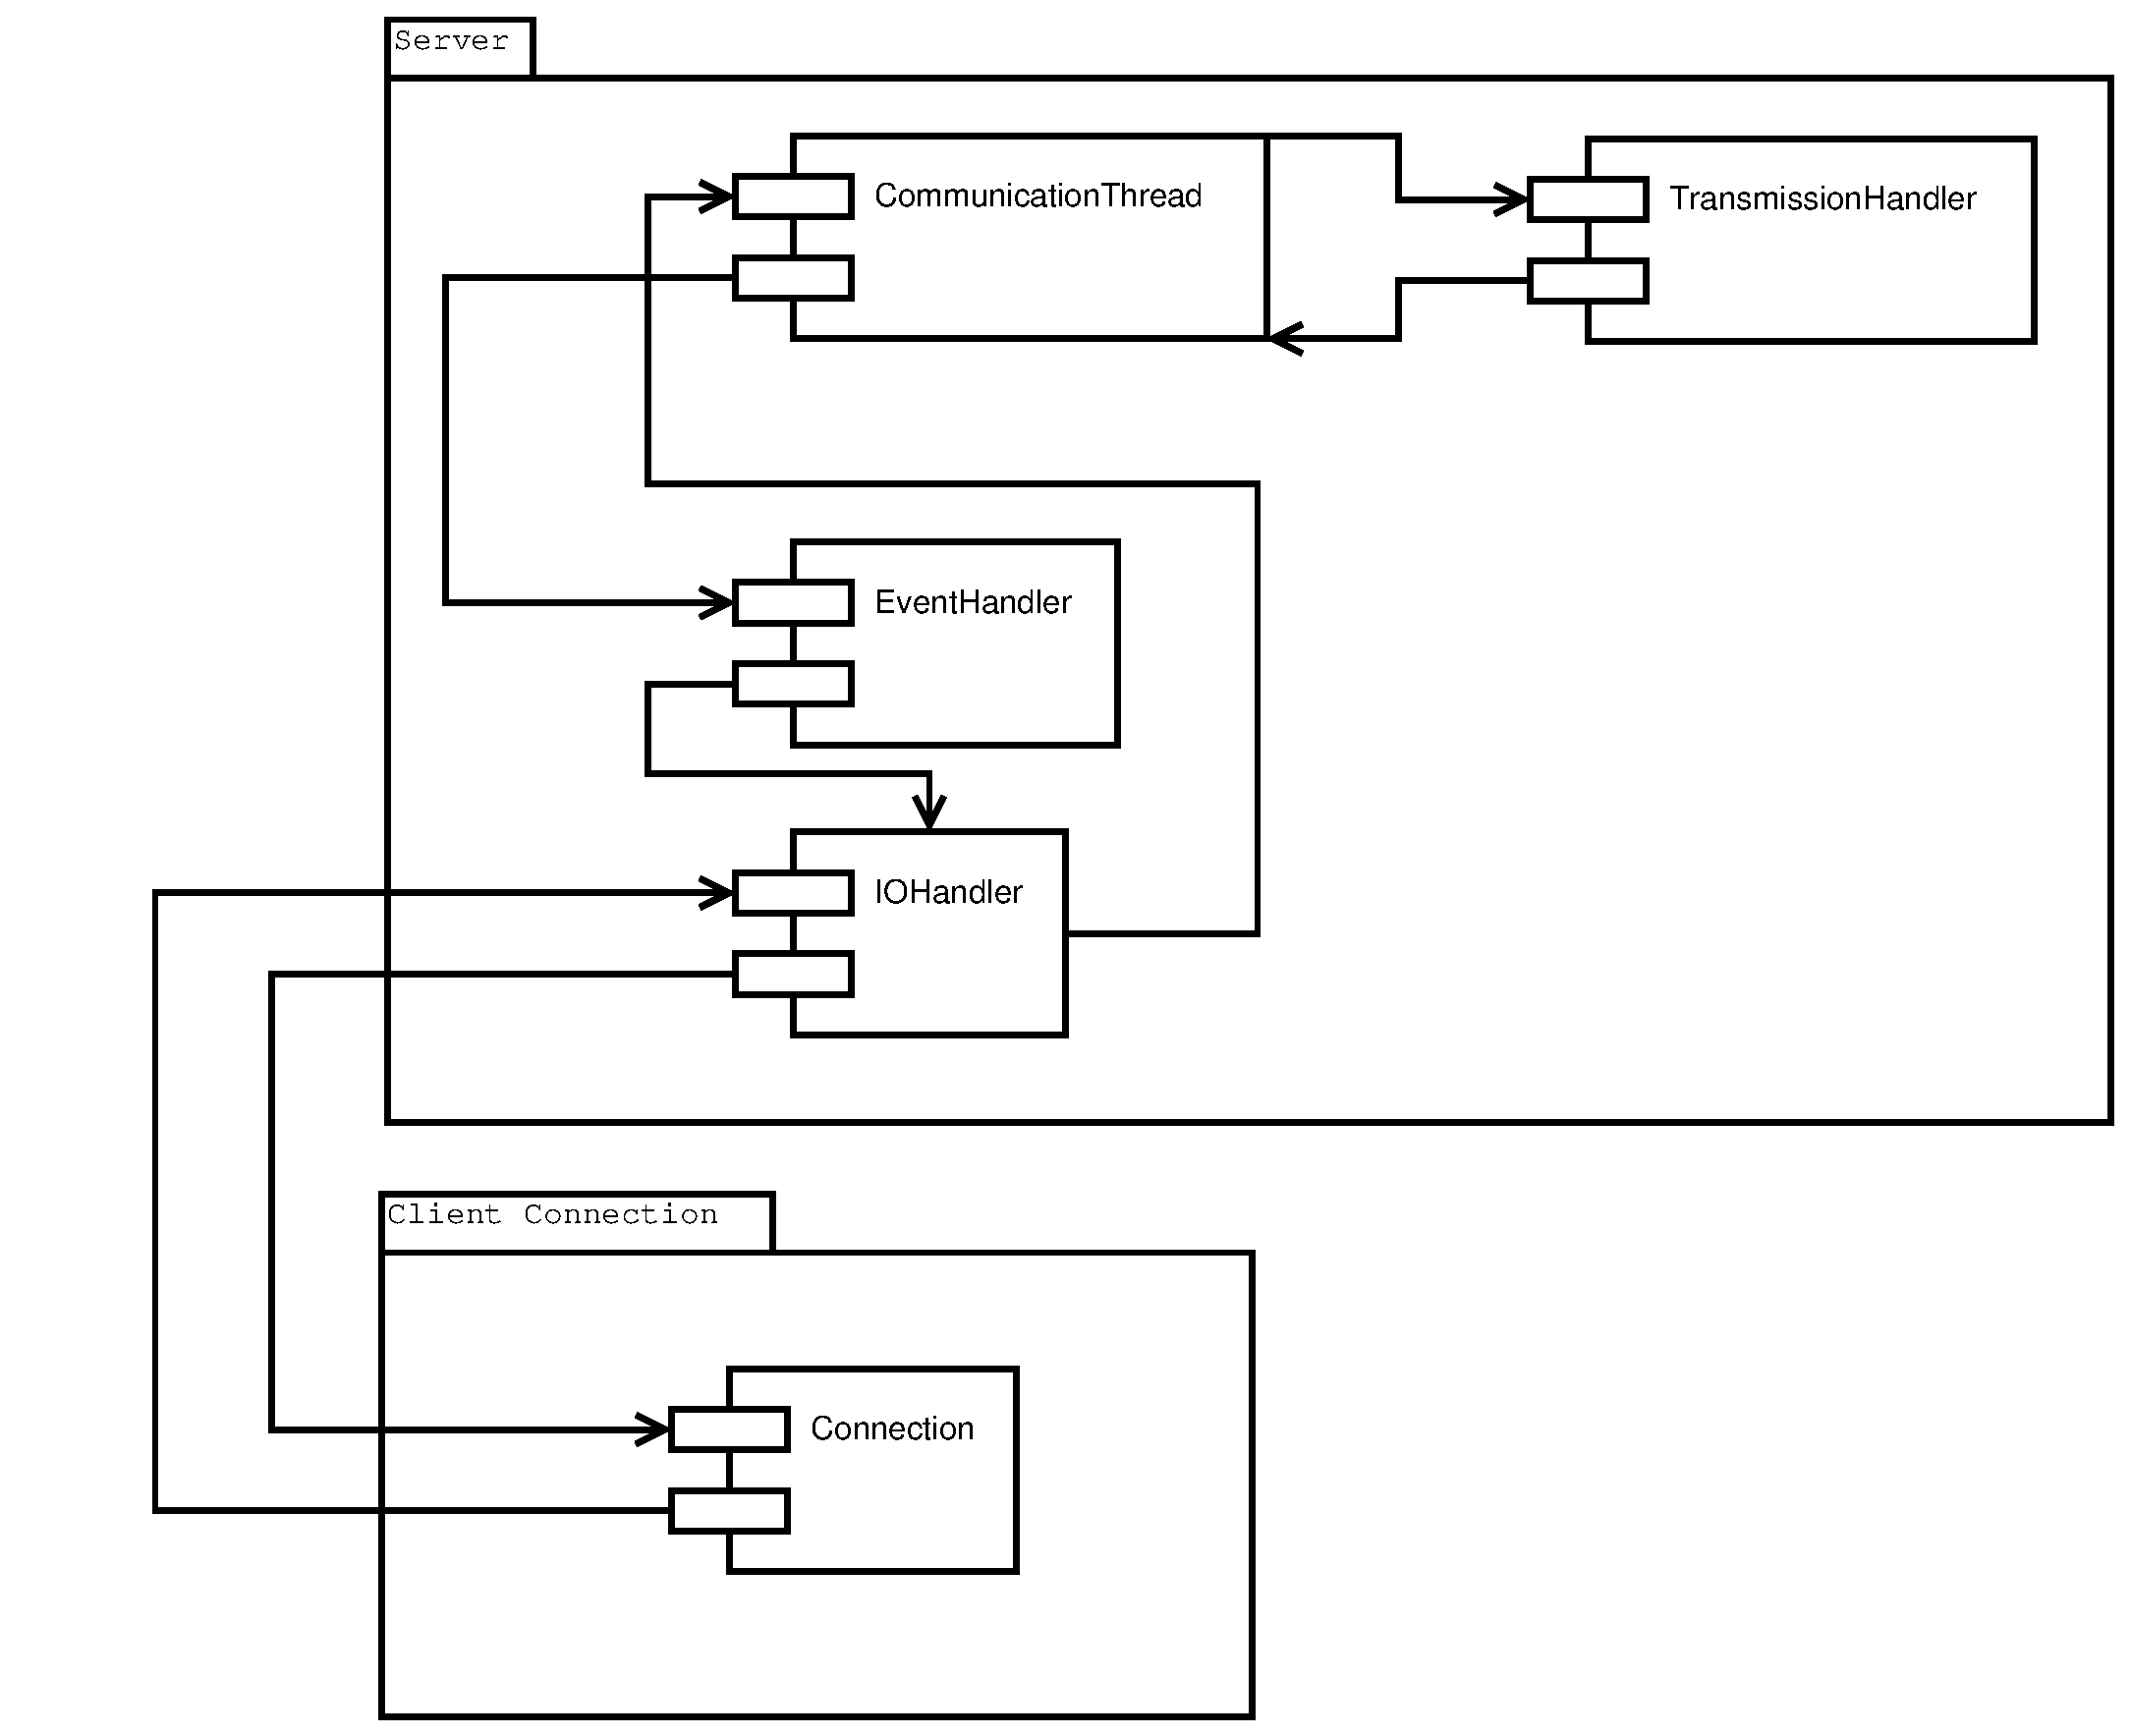
\includegraphics[scale=0.30]{images/requestCommit.eps} %FIXME epstopdf package fucker, men har ikke ændret noget da den fucker fuldstændig, genere ikke pdfen??!?!
	\caption{A diagram illustrating how a request or a commit event is processed.}
	\label{fig:IOCR}
\end{figure}
      \subsubsection{Queue and Query handling} %Martin
	  \label{QQHandling}
	    The following sections presents an overview of the queue and query implementation of Savannah's server software.
\subsubsection{Queue}

As mentioned in \autoref{sect:ssArchAndDesign} Savannah is designed around a producer-consumer pattern centered on a FIFO queue, implemented in the \code{EventQueue} class.
The UML diagram in \autoref{figure:EventUML} shows the event queue implementation and closely related classes.
The event queue is a \code{LinkedList<Event>} object instantiated as a \code{Queue<Event>}, this instantiation defaults to a FIFO queue through
the \code{queue.add(event)} and \code{queue.remove()} methods. \code{EventQueue} is implemented as a singleton to ensure that Savannah never has access to more than one queue.
Events are implemented through the \code{Event} interface that \code{RequestEvent} and \code{CommitEvent} implements.
Finally the \code{EventHandler} class is responsible for removing events from the queue and make sure they are processed by the server. It is started as a thread and
continuously probes the queue for content. All queue access is synchronized, through the use of the Java \code{synchronized} keyword, to avoid race conditions.

\begin{figure}[H]
 \centering
  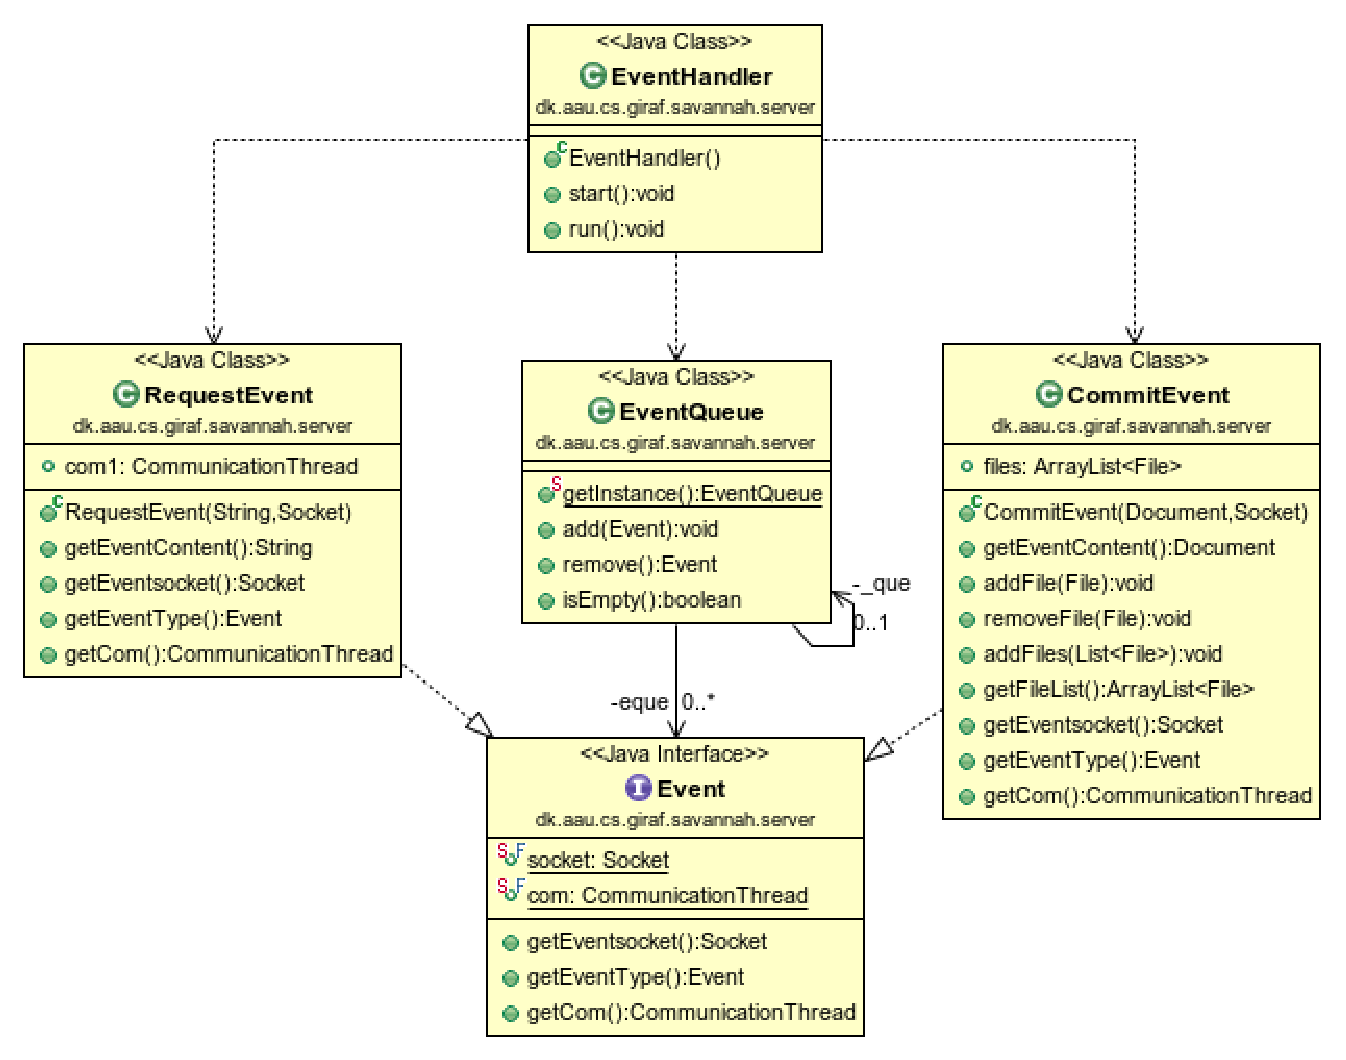
\includegraphics[scale=0.65]{images/EventQueue}
  \caption{EventQueue UML diagram.}
  \label{figure:EventUML}
\end{figure}

An event contains a reference to the socket on which the connection was made and the event content, which is either an XML document or a \code{String} containing certificates
needed to query profiles from the database.

\subsubsection{Query creation and handling}

The UML diagram in \autoref{figure:queryUML} shows the \code{EventHandler} and related classes for building SQL queries, querying the database, and building XML documents.
The \code{Eventhandler} instantiates a \code{RequestHandler} and a \code{CommitHandler}, which are responsible for handling request- or commit events.
Each of the handlers instatiate a \code{QueryBuilder} and a \code{QueryHandler}. The \code{QueryBuilder} creates SQL queries based on the event content. The queries are forwarded to the \code{QueryHandler}
that interacts with the database and, if the event is a \code{RequestEvent}, returns a \code{ResultSet} object. Finally the \code{Resultset} object is forwarded to the \code{XMLBuilder} that builds an sw6ml document,
in \code{String} form, that can be returned to the requesting party. 
\begin{figure}[H]
 \centering
  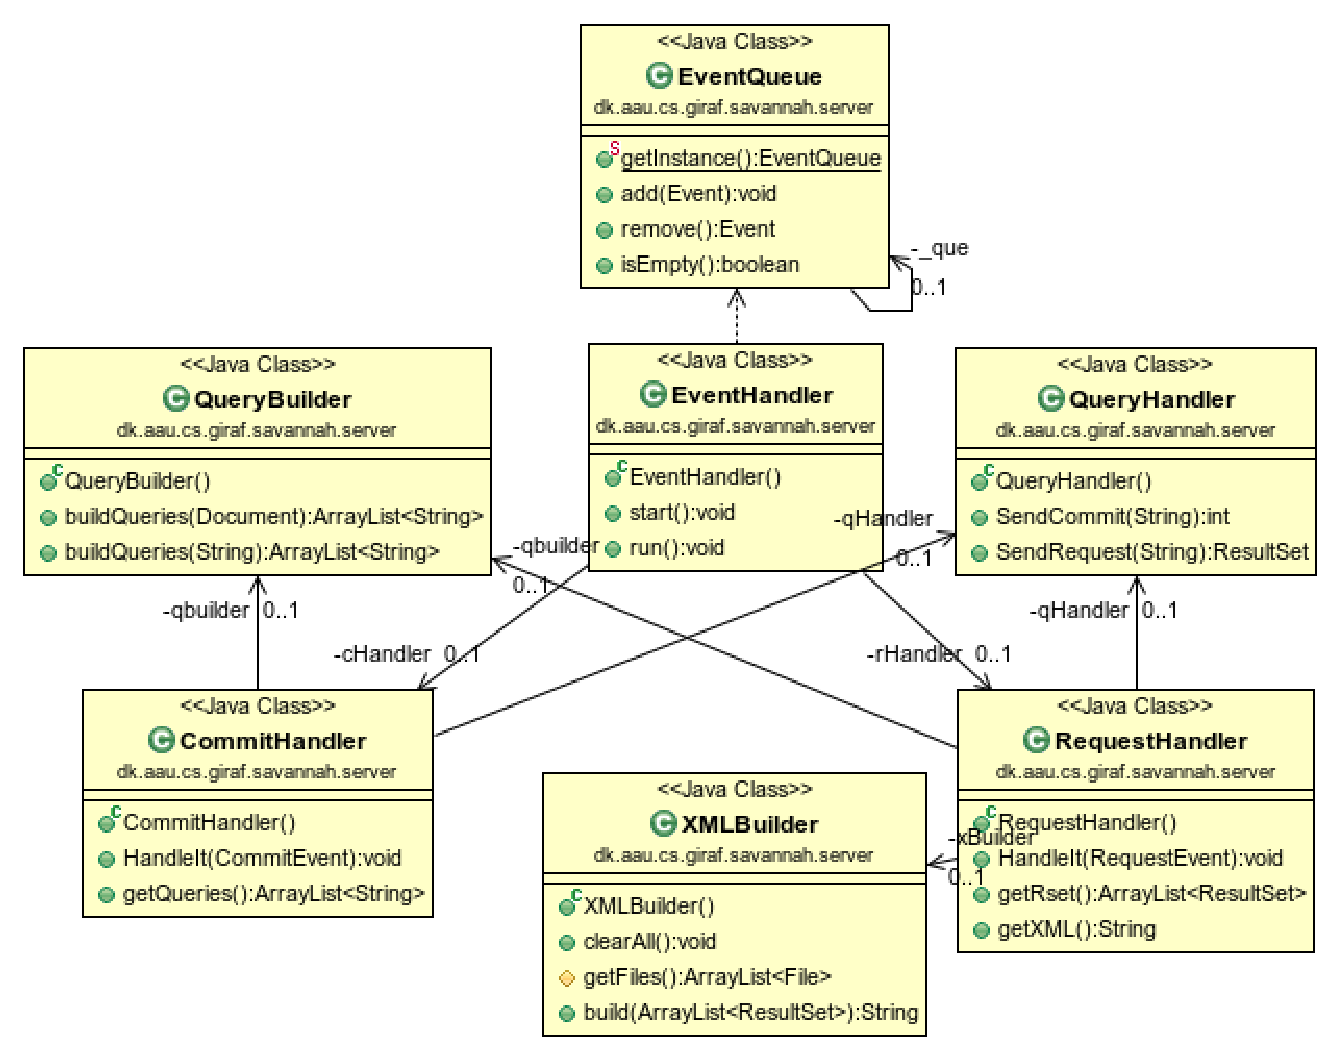
\includegraphics[scale=0.65]{images/queryhandling}
  \caption{Query handling UML diagram.}
  \label{figure:queryUML}
\end{figure}


    \subsection{Test}
      \subsubsection{JUnit}
      \subsubsection{Other test}

\chapter{Recapitulation}
  \section{Conclusion}
  \section{Future work}
  \section{Multi project} % skal den være med

\appendix
	\chapter{Appendix}
	\section{MySQL Code}
	\label{MySQLcode}
		%appendixCreateSQL.tex
\begin{lstlisting}[language=SQL,breaklines=true, label=createAuthUsers, caption=Create AuthUsers, float]
  CREATE  TABLE `04`.`AuthUsers` (

  `certificate` VARCHAR(512) NOT NULL ,

  `idUser` INT NOT NULL AUTO_INCREMENT ,
  
  `aRole` INT NOT NULL,
    
  `username` VARCHAR(45) UNIQUE NOT NULL,
  
  `password` VARCHAR(45) NOT NULL,

  PRIMARY KEY (`certificate`) ,

  UNIQUE INDEX `idUser_UNIQUE` (`idUser` ASC) );
\end{lstlisting}

\begin{lstlisting}[language=SQL,breaklines=true, label=createApps, caption=Create Apps]
  
  CREATE  TABLE `04`.`Apps` (

  `idApp` INT NOT NULL AUTO_INCREMENT,

  `name` VARCHAR(45) NOT NULL ,

  `version` VARCHAR(45) NOT NULL ,
  
  `icon` VARCHAR(45) NOT NULL,
  
  `package` VARCHAR(45) NOT NULL,
  
  `activity` VARCHAR(45) NOT NULL,

  PRIMARY KEY (`idApp`) );
\end{lstlisting}

\begin{lstlisting}[language=SQL,breaklines=true, label=createTags, caption=Create Tags]
CREATE  TABLE `04`.`Tags` (

  `idTags` INT NOT NULL AUTO_INCREMENT,

  `caption` VARCHAR(45) NOT NULL ,

  PRIMARY KEY (`idTags`) ,

  UNIQUE INDEX `caption_UNIQUE` (`caption` ASC) );

\end{lstlisting}

\begin{lstlisting}[language=SQL,breaklines=true, label=createProfile, caption=Create Profile]
CREATE  TABLE `04`.`Profile` (

  `idProfile` INT NOT NULL ,

  `firstname` VARCHAR(45) NOT NULL ,

  `surname` VARCHAR(45) NOT NULL ,

  `middlename` VARCHAR(45) NULL ,

  `pRole` INT NOT NULL ,

  `phone` BIGINT NOT NULL ,

  `picture` VARCHAR(45) NULL ,

  `settings` BLOB NULL ,
  
  FOREIGN KEY (`idProfile` )

  REFERENCES `04`.`AuthUsers` (`idUser` ) on delete cascade,

  PRIMARY KEY (`idProfile`) );
\end{lstlisting}

\begin{lstlisting}[language=SQL,breaklines=true, label=createListOfApps, caption=Create ListOfApps]
CREATE  TABLE `04`.`ListOfApps` (

  `idApp` INT NOT NULL ,

  `idProfile` INT NOT NULL ,
  
  `setting` BLOB,
  
  `stats` BLOB,
  
  FOREIGN KEY (`idApp` )

  REFERENCES `04`.`Apps` (`idApp` ),
  
  FOREIGN KEY (`idProfile` )

  REFERENCES `04`.`Profile` (`idProfile` ) ON DELETE CASCADE,

  PRIMARY KEY (`idApp`,`idProfile`) );

\end{lstlisting}

\begin{lstlisting}[language=SQL,breaklines=true, label=createDepartment, caption=Create Department]
CREATE  TABLE `04`.`Department` (

  `idDepartment` INT NOT NULL ,

  `name` VARCHAR(45) NOT NULL ,

  `address` VARCHAR(45) NOT NULL ,

  `phone` BIGINT NOT NULL ,

  `email` VARCHAR(45) NOT NULL ,
  
  FOREIGN KEY (`idDepartment` )

  REFERENCES `04`.`AuthUsers` (`idUser` ),

  PRIMARY KEY (`idDepartment`) );

\end{lstlisting}

\begin{lstlisting}[language=SQL,breaklines=true, label=createHasDepartment, caption=Create HasDepartment]
CREATE  TABLE `04`.`HasDepartment` (

  `idProfile` INT NOT NULL ,

  `idDepartment` INT NOT NULL ,
  
  FOREIGN KEY (`idProfile` )

  REFERENCES `04`.`Profile` (`idProfile` ) ON DELETE CASCADE,

  FOREIGN KEY (`idDepartment` )

  REFERENCES `04`.`Department` (`idDepartment` ),


  PRIMARY KEY (`idProfile`, `idDepartment`) );

\end{lstlisting}

\begin{lstlisting}[language=SQL,breaklines=true, label=createHasGuardian, caption=Create HasGuardian]
CREATE  TABLE `04`.`HasGuardian` (

  `idGuardian` INT NOT NULL ,

  `idChild` INT NOT NULL ,
  
  FOREIGN KEY (`idGuardian` )

  REFERENCES `04`.`Profile` (`idProfile` ) on delete cascade,
  
  FOREIGN KEY (`idChild` )

  REFERENCES `04`.`Profile` (`idProfile` ) on delete cascade,

  PRIMARY KEY (`idGuardian`,`idChild`) );

\end{lstlisting}

\begin{lstlisting}[language=SQL,breaklines=true, label=createHasSubDepartment, caption=Create HasSubDepartment]
CREATE  TABLE `04`.`HasSubDepartment` (

  `idDepartment` INT NOT NULL ,

  `idSubDepartment` INT NOT NULL ,
  
  FOREIGN KEY (`idDepartment` )

  REFERENCES `04`.`Department` (`idDepartment` ),
  
  FOREIGN KEY (`idSubDepartment` )

  REFERENCES `04`.`Department` (`idDepartment` ),

  PRIMARY KEY (`idDepartment`, `idSubDepartment`) );

\end{lstlisting}

\begin{lstlisting}[language=SQL,breaklines=true, label=createMedia, caption=Create Media]
CREATE  TABLE `04`.`Media` (

  `idMedia` INT NOT NULL AUTO_INCREMENT,

  `mPath` VARCHAR(45) NOT NULL ,

  `name` VARCHAR(45) NOT NULL ,

  `mPublic` TINYINT NOT NULL ,

  `mType` VARCHAR(45) NOT NULL ,

  `ownerID` INT NOT NULL ,
  
  FOREIGN KEY (`OwnerID` )

  REFERENCES `04`.`AuthUsers` (`idUser` )  ON DELETE CASCADE,

  PRIMARY KEY (`idMedia`) );

\end{lstlisting}

\begin{lstlisting}[language=SQL,breaklines=true, label=createHasTag, caption=Create HasTag]
CREATE  TABLE `04`.`HasTag` (

  `idMedia` INT NOT NULL ,

  `idTag` INT NOT NULL ,
  
  FOREIGN KEY (`idMedia` )

  REFERENCES `04`.`Media` (`idMedia` ) on delete cascade,
  
  FOREIGN KEY (`idTag` )

  REFERENCES `04`.`Tags` (`idTags` ),

  PRIMARY KEY (`idMedia`, `idTag`) );

\end{lstlisting}

\begin{lstlisting}[language=SQL,breaklines=true, label=createHasLink, caption=Create HasLink]
CREATE  TABLE `04`.`HasLink` (

  `idMedia` INT NOT NULL ,

  `idSubMedia` INT NOT NULL ,
  
  FOREIGN KEY (`idMedia` )

  REFERENCES `04`.`Media` (`idMedia` ) on delete cascade,
  
  FOREIGN KEY (`idSubMedia` )

  REFERENCES `04`.`Media` (`idMedia` ) on delete cascade,

  PRIMARY KEY (`idMedia`, `idSubMedia`) );

\end{lstlisting}

\begin{lstlisting}[language=SQL,breaklines=true, label=createMediaProfileAccess, caption=Create MediaProfileAccess]
CREATE  TABLE `04`.`MediaProfileAccess` (

  `idProfile` INT NOT NULL ,

  `idMedia` INT NOT NULL ,
  
  FOREIGN KEY (`idProfile` )

  REFERENCES `04`.`Profile` (`idProfile` ) ON DELETE CASCADE,
  
  FOREIGN KEY (`idMedia` )

  REFERENCES `04`.`Media` (`idMedia` ) ON DELETE CASCADE,

  PRIMARY KEY (`idProfile`, `idMedia`) );

\end{lstlisting}

\begin{lstlisting}[language=SQL,breaklines=true, label=createMediaDepartmentAccess, caption=Create MediaDepartmentAccess]
CREATE  TABLE `04`.`MediaDepartmentAccess` (

  `idDepartment` INT NOT NULL ,

  `idMedia` INT NOT NULL ,
  
  FOREIGN KEY (`idDepartment` )

  REFERENCES `04`.`Department` (`idDepartment` ),
  
  FOREIGN KEY (`idMedia` )

  REFERENCES `04`.`Media` (`idMedia` ),

  PRIMARY KEY (`idDepartment`, `idMedia`) );

\end{lstlisting}

	\section{ER Diagram}
	\label{errDiagram}
		%workbenchERRdiagram.tex
\begin{figure}[H]
	\centering
		\includegraphics[width=1.00\textwidth]{images/workbenchWrong.png}
	\caption{The ERR diagram as MySQL Workbench generates it}
	\label{fig:workbenchWrong}
\end{figure}

	\section{Class Diagrams}
	\label{app:Class-diagrams}
		%appendixIOHandler.tex

\begin{figure}[H]
	\centering
		\includegraphics[scale=0.70]{images/IOHandler.PNG}
	\caption{Class-diagram of the \code{IOHandler} class}
	\label{fig:app:IOHandler}
\end{figure}

\begin{figure}[H]
	\centering
		\includegraphics[scale=0.70]{images/Connection.PNG}
	\caption{Class-diagram of the \code{Connection} class}
	\label{fig:app:Connection}
\end{figure}

\begin{figure}[H]
	\centering
		\includegraphics[scale=0.70]{images/TransmissionHandler.PNG}
	\caption{Class-diagram of the \code{TransmissionHandler} class}
	\label{fig:app:TransmissionHandler}
\end{figure}
        \chapter{Notes from Interview}
\label{InterviewMette}
\textit{This is notes from an interview with Mette Als Andreasen, an educator at Birken in Langholt, Denmark.}

N\aa{}r tiden l\o{}ber ud (kristian har tage et billede):\\
F\ae{}rdig - symbol\\
G\aa{} til skema - symbol\\
Taget fra boardmaker\\

Kunne v\ae{}re godt hvis man kunne s\ae{}tte egne billeder ind som start/stop symboler.\\


R\o{}d farve $=$ nej, stop, aflyst.\\

De har s\aa{}dan et ur p\aa{} 60 minutter hvor tid tilbage er markeret med r\o{}d, og s\aa{} bipper den lige kort n\aa{}r den er f\ae{}rdig.\\
  Det ville v\ae{}re fint hvis de kunne bruge sort/hvid til dem der ikke kan h\aa{}ndtere farver, men ogs\aa{} kan v\ae{}lge farver.\\

Stop-ur:\\
en fast timer p\aa{} 60 minutter $+$ en customizable som ikke ser helt magen til ud, som f.eks, kan v\ae{}re p\aa{} 5, 10 eller 15 minutter for en hel cirkel.\\

timeglas:\\
skift farve p\aa{} timeglassene, men ikke n\o{}dvendigvis g\o{}re dem st\o{}rre. Kombinere med mere/mindre sand. Eventuelt kombinere med et lille digitalt ur, til dem der har brug for det, skal kunne sl\aa{}es til og fra.\\

Dags-plan:\\
ikke s\ae{}rlig relevant til de helt sm\aa{} og ikke s\ae{}rligt velfungerende b\o{}rn. Men kunne v\ae{}re rigtig godt til de lidt \ae{}ldre.\\
   En plan g\aa{}r oppefra og ned, og hvis der s\aa{} skal specificeres noget ud til aktiviteterne, s\aa{} er det fra venstre mod h\o{}jre ud fra det nedadg\aa{}ende skema.\\

Til parrot:\\
Godt med rigtige billeder af tingene, som p\ae{}dagogerne selv kan tage, eventuelt ogs\aa{} af aktiviteter, s\aa{} pedagogerne kan have billeder af aktiviter som de kan liste efter skeamet.\\

Der var mange skemaer rundt omkring, og der henviser det sidste billede i r\ae{}kken til n\ae{}ste skema, som h\ae{}nger f.eks. p\aa{} badev\ae{}relset eller i garderoben.
\begin{figure}%
	\begin{center}
	\includegraphics[width=\textwidth]{input/appendices/invitation_to_usability_test.pdf}
	\end{center}
\caption{Invitation sent to the test persons of the usability test.}%
\label{appendice:usability_test}%
\end{figure}
\bibliographystyle{plainnat}
\bibliography{bib}

\appendix

\end{document}
